\documentclass[convert={density=300,size=1080x800,outext=.png}]{standalone}
\usepackage{tkz-graph}
\usetikzlibrary{arrows,positioning,shapes,shapes.multipart,patterns,mindmap,shadows}
\usepackage{xcolor}
\usepackage{helvet}
\renewcommand{\familydefault}{\sfdefault}


\begin{document}

\footnotesize
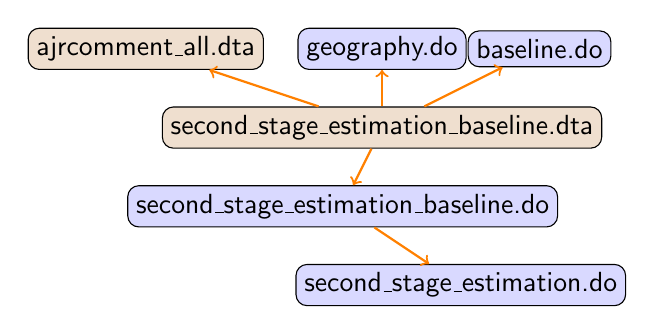
\begin{tikzpicture}[every node/.style={
    rectangle,
    rounded corners,
    inner sep=3pt,
    draw,
    fill=brown!25
}]
    \node (ajrcomment_all_dta) [shift={(2, 0)}]
    {
        ajrcomment\_all.dta
    };



    \node (geography_do) [fill=blue!15, shift={(5, 0)}]
    {
        geography.do
    };
    \node (baseline_do) [fill=blue!15, shift={(7, 0)}]
    {
        baseline.do
    };




    \node (second_stage_estimation_baseline_dta) [shift={(5, -1)}]
    {
        second\_stage\_estimation\_baseline.dta
    };



    \node (second_stage_estimation_baseline_do) [fill=blue!15, shift={(4.5, -2)}]
    {
        second\_stage\_estimation\_baseline.do
    };


    \node (second_stage_estimation_do) [fill=blue!15, shift={(6, -3)}]
    {
        second\_stage\_estimation.do
    };




    \draw[->, orange, thick] (second_stage_estimation_baseline_dta) to (second_stage_estimation_baseline_do);
    \draw[->, orange, thick] (second_stage_estimation_baseline_dta) to (geography_do);
    \draw[->, orange, thick] (second_stage_estimation_baseline_dta) to (ajrcomment_all_dta);
    \draw[->, orange, thick] (second_stage_estimation_baseline_dta) to (baseline_do);
    \draw[->, orange, thick] (second_stage_estimation_baseline_do) to (second_stage_estimation_do);


\end{tikzpicture}

\end{document}

